%!TEX root = ../problems.tex
\begin{figure}[h!]
\centering
\begin{minipage}{0.4\textwidth}
\centering
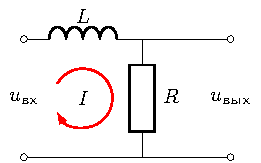
\includegraphics[width=\linewidth]{chem/task2}
\caption{$RL$--контур}
\label{fig:4figsA}
\end{minipage}
\qquad
\begin{minipage}{0.4\textwidth}
\centering
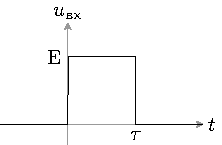
\includegraphics[width=\linewidth]{ris/task4_input}
\caption{Входное напряжение}
\label{fig:4figsB}
\end{minipage}
\end{figure}

\begin{task}
	Определить отклик $u_\out(t)$ $RL$-цепи, изображенной на рисунке, на воздействие двух прямоугольных импульсов длительностью $\tau$. 
	Нарисуйте график отклика. 
	Какова переходная характеристика цепи? 
	При выполнении какого условия будет осуществляться приближённое дифференцирование входной цепи?
	Решить задачу с ненулевыми начальными условиями.
\end{task}
\begin{proof}[\rm{\textbf{Решение}}]
Найдем образ входного импульса преобразованием Лапласа: 
\begin{equation}
	u_\in(t)=A[\H(t)-\H(t- \tau)]+A[\H(t-2 \tau)-\H(t-3 \tau)]
\end{equation}
\begin{equation}
	u_\in(t)\LT \frac{A}{p}\qty(1-e^{-p \tau}+e^{-2p \tau}-e^{-3p \tau})
\end{equation}

Надо учесть, что в контуре могут быть заданы начальные условия - напряжение на индуктивности $u_L(0)=u_0$. Его образ $u_L(0) \LT \frac{pLi_0}{p} $. Это напряжение можно учесть как ещё одну стороннюю ЭДС.

Обозначим суммарный ток в контуре за $I(p)$. Тогда, так как сумма падений напряжения на каждом элементе равна нулю, получим следующее выражение:
\begin{equation}
	U_\in+Li_0=(pL+R)i_0
\end{equation}

Откуда выразим ток $I$:
\begin{equation}
	I(p)=
	\frac{\frac{A}{p}\qty(1-e^{-p \tau}+e^{-2p \tau}-e^{-3p \tau})+Li_0}
	{pL+R}
\end{equation}
После простых алгебраических преобразований получим:
\begin{equation}
	I(p)=
	\frac{\frac AL }{p+\frac{R}{L}}-
	\frac{\frac AL e^{-p\tau}}{p+\frac{R}{L}}+
	\frac{\frac AL e^{-2p\tau}}{p+\frac{R}{L}}-
	\frac{\frac AL e^{-3p\tau}}{p+\frac{R}{L}}+
	\frac{i_0}{p+\frac{R}{L}}
\end{equation}
Отсюда можем получить напряжение на выходе:
\begin{equation}
	U_\out(p)=
	\frac{A\frac RL }{p+\frac{R}{L}}-
	\frac{A\frac RL e^{-p\tau}}{p+\frac{R}{L}}+
	\frac{A\frac RL e^{-2p\tau}}{p+\frac{R}{L}}-
	\frac{A\frac RL e^{-3p\tau}}{p+\frac{R}{L}}+
	\frac{i_0R}{p+\frac{R}{L}}
\end{equation}
Используем свойства преобразования Лапласа:
\begin{gather}
	\frac{\alpha}{p(p+\alpha)}\LT (1-e^{-\alpha t})\H(t)\\
	\frac{1}{(p+\alpha)}\LT e^{-\alpha t}\H(t)\\
	e^{{-p\tau}}F(p) \LT f(t-\tau)\H(t-\tau), \qq{где} F(p) \LT f(t)
\end{gather}
Произведем преобразование:
\begin{gather}
	U(t)=A [ 
	(1-e^{-\frac{R}{L}t})\H(t)-(1-e^{-\frac{R}{L}(t- \tau)})\H(t- \tau)+(1-e^{-\frac{R}{L}(t- 2\tau)})\H(t- 2\tau)-\\
	(1-e^{-\frac{R}{L}(t- 3\tau)})\H(t- 3\tau)]+i_0Re^{-\frac{R}{L}t}\H(t)
\end{gather}


\begin{figure}[h!]
	\centering
	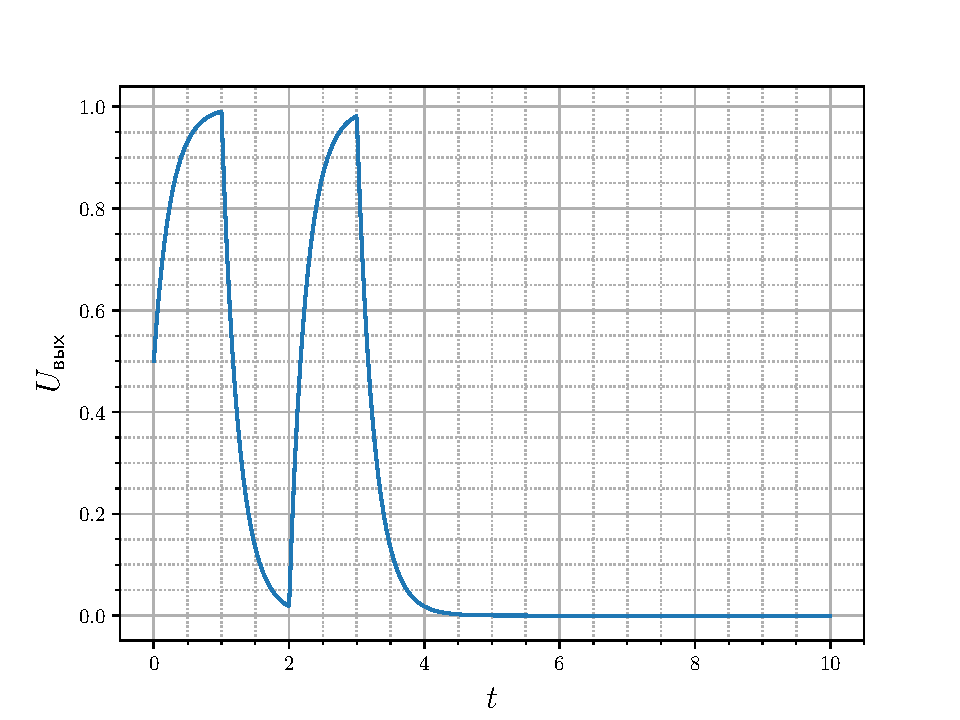
\includegraphics[width=0.7\linewidth]{ris/task12_out}
	\caption{Решение при $A=1, i_0R=0.5, \tau=5, R/L=4, \tau=1$}
	\label{fig:12.2}
\end{figure}

\begin{equation}
	u(t)=(E-u_0)\H(t)\exp{-\frac{t}{CR}}-E \exp{-\frac{t- \tau	}{CR}}\H(t-\tau )
\end{equation} 
График решения при при $A=1, i_0R=0.5, \tau=5, R/L=4, \tau=1$ изображен на рис. \ref{fig:12.2}


\paragraph{Условие интегрирования} 
% Как нетрудно догадаться,
% \begin{equation}
% 	u_\in=u_C+u_R=\frac{q}{C}+IR
% \end{equation}
% Продифференцируем это выражение:
% \begin{equation}
% 	\dv{u_\in}{t}=
% 	\frac{1}{CR}\underbrace{IR}_{u_R\equiv u_\out}+
% 	\underbrace{\dv{I}{t}R}_{\dv{u_R}{t}}
% \end{equation}
% Если будет выполнено условие
% \begin{equation}
% 	\abs{\dv{u_R}{t}} \ll \abs{\frac{1}{CR} u_R}
% \end{equation}
% Тогда будет видно, что цепочка осуществляет дифференцирование:
% \begin{equation}
% 	u_\out=CR\dv{u_\in}{t}=\tau_{\text{цепи}}\dv{u_\in}{t}
% \end{equation}




% Выясним смысл неравенства модулей на примере гармонических сигналов. Пусть входное напряжение гармоническое $u_\in=u_0e^{i\omega t}$. Тогда ток в контуре: $I=I_0 e^{i\omega t}$, где $I_0=\frac{u_0}{\frac{1}{i \omega C}+R}$, и неравенство можно переписать (учтем, что $u_C=\frac{I}{i \omega C}=\frac{Ie^{i \omega t}}{i \omega C}$):
% \begin{equation}
% 	\abs{ I_0R \cdot i\omega\cdot e^{i\omega t}}\ll
% 		\abs{\frac{1}{\tau_\text{цепи}}{I_0}R \cdot e^{i\omega t}}
% 	\quad \Rightarrow \quad
% 	\omega \ll {\frac{1}{\tau_\text{цепи}}}
% 	\quad \Rightarrow \quad
% 	T \gg \tau_\text{цепи}
% \end{equation}
% Таким образом, дифференцирование сигнала <<чистое>> для таких частот, период которых много больше постоянной времени цепи. Отсюда следует <<вилка выбора>> дифференцирующей цепочки: если мы будем расширять частотный диапазон <<чистого>> дифференцирования уменьшением постоянной времени, то амплитуда на выходе цепочки будет падать, и наоборот.


\end{proof}